%%
%% This is file `sample-manuscript.tex',
%% generated with the docstrip utility.
%%
%% The original source files were:
%%
%% samples.dtx  (with options: `manuscript')
%% 
%% IMPORTANT NOTICE:
%% 
%% For the copyright see the source file.
%% 
%% Any modified versions of this file must be renamed
%% with new filenames distinct from sample-manuscript.tex.
%% 
%% For distribution of the original source see the terms
%% for copying and modification in the file samples.dtx.
%% 
%% This generated file may be distributed as long as the
%% original source files, as listed above, are part of the
%% same distribution. (The sources need not necessarily be
%% in the same archive or directory.)
%%
%% The first command in your LaTeX source must be the \documentclass command.
%%%% Small single column format, used for CIE, CSUR, DTRAP, JACM, JDIQ, JEA, JERIC, JETC, PACMCGIT, TAAS, TACCESS, TACO, TALG, TALLIP (formerly TALIP), TCPS, TDSCI, TEAC, TECS, TELO, THRI, TIIS, TIOT, TISSEC, TIST, TKDD, TMIS, TOCE, TOCHI, TOCL, TOCS, TOCT, TODAES, TODS, TOIS, TOIT, TOMACS, TOMM (formerly TOMCCAP), TOMPECS, TOMS, TOPC, TOPLAS, TOPS, TOS, TOSEM, TOSN, TQC, TRETS, TSAS, TSC, TSLP, TWEB.
% \documentclass[acmsmall]{acmart}
\documentclass[sigchi,authordraft]{acmart}

%% 追加
\usepackage{bm}
\newcommand\figref[1]{\textbf{Figure~\ref{fig:#1}}}
\newcommand\tabref[1]{\textbf{Table~\ref{tab:#1}}}
\usepackage{url}
\usepackage{color}
\usepackage{multirow}
\usepackage[subrefformat=parens]{subcaption}
\captionsetup{compatibility=false}
%% ここまで

%%%% Large single column format, used for IMWUT, JOCCH, PACMPL, POMACS, TAP, PACMHCI
% \documentclass[acmlarge,screen]{acmart}

%%%% Large double column format, used for TOG
% \documentclass[acmtog, authorversion]{acmart}

%%%% Generic manuscript mode, required for submission
%%%% and peer review
% \documentclass[manuscript,screen,review]{acmart}
%% Fonts used in the template cannot be substituted; margin 
%% adjustments are not allowed.
%%
%% \BibTeX command to typeset BibTeX logo in the docs
\AtBeginDocument{%
  \providecommand\BibTeX{{%
    \normalfont B\kern-0.5em{\scshape i\kern-0.25em b}\kern-0.8em\TeX}}}

%% Rights management information.  This information is sent to you
%% when you complete the rights form.  These commands have SAMPLE
%% values in them; it is your responsibility as an author to replace
%% the commands and values with those provided to you when you
%% complete the rights form.
\setcopyright{acmcopyright}
\copyrightyear{2018}
\acmYear{2018}
\acmDOI{10.1145/1122445.1122456}

%% These commands are for a PROCEEDINGS abstract or paper.
\acmConference[Woodstock '18]{Woodstock '18: ACM Symposium on Neural
  Gaze Detection}{June 03--05, 2018}{Woodstock, NY}
\acmBooktitle{Woodstock '18: ACM Symposium on Neural Gaze Detection,
  June 03--05, 2018, Woodstock, NY}
\acmPrice{15.00}
\acmISBN{978-1-4503-XXXX-X/18/06}


%%
%% Submission ID.
%% Use this when submitting an article to a sponsored event. You'll
%% receive a unique submission ID from the organizers
%% of the event, and this ID should be used as the parameter to this command.
%%\acmSubmissionID{123-A56-BU3}

%%
%% The majority of ACM publications use numbered citations and
%% references.  The command \citestyle{authoryear} switches to the
%% "author year" style.
%%
%% If you are preparing content for an event
%% sponsored by ACM SIGGRAPH, you must use the "author year" style of
%% citations and references.
%% Uncommenting
%% the next command will enable that style.
%%\citestyle{acmauthoryear}

%%
%% end of the preamble, start of the body of the document source.
\begin{document}

%%
%% The "title" command has an optional parameter,
%% allowing the author to define a "short title" to be used in page headers.
\title{Pulse Wave Generation Method for PPG by using Display}

%%
%% The "author" command and its associated commands are used to define
%% the authors and their affiliations.
%% Of note is the shared affiliation of the first two authors, and the
%% "authornote" and "authornotemark" commands
%% used to denote shared contribution to the research.

\author{Atsuhiro Fujii}
\affiliation{%
  \institution{Ritsumeikan University}
   \city{Shiga}
   \country{Japan}
}
\email{atsuhiro.fujii@iis.ise.ritsumei.ac.jp}

\author{Kazuya Murao}
\affiliation{%
  \institution{Ritsumeikan University / Japan Science and Technology Agency, PRESTO}
   \city{Shiga}
   \country{Japan}
}
\email{murao@cs.ritsumei.ac.jp}

\author{Naoji Matsuhisa}
\affiliation{%
  \institution{Keio University / Japan Science and Technology Agency, PRESTO}
   \city{Kanagawa}
   \country{Japan}
}
\email{naoji@keio.jp}

%%
%% By default, the full list of authors will be used in the page
%% headers. Often, this list is too long, and will overlap
%% other information printed in the page headers. This command allows
%% the author to define a more concise list
%% of authors' names for this purpose.
\renewcommand{\shortauthors}{Fujii and Murao}

%%
%% The abstract is a short summary of the work to be presented in the
%% article.
\begin{abstract}
  The extensive research on wearable devices has led to devices with various shapes and mounting locations. Wearable devices are often used to record the user's biometric information, and methods have been proposed to detect physical abnormalities from the acquired data. Among various kinds of biometric data, pulse data has been used in methods such as heart rate monitoring and emotion recognition. The most common type of pulse sensor uses photoplethysmography (PPG), which irradiates a green LED on the skin and measures pulse data from changes in the light reflected from blood vessels. PPG sensors have been implemented in commercially available wearable devices such as smartwatches. However, a PPG sensor requires blood flow for data acquisition, and when a smartwatch is worn on an artificial body part such as a prosthetic hand or a robotic arm, data cannot be acquired because there is no blood flow. In this study, we propose a method that enables a PPG sensor to measure arbitrary pulse data by using a display. If this method is successful, it will enable pulse data measured at the junction of a living limb and an artificial limb to be input to the display; then, a smartwatch attached to the artificial limb will read the same pulse data. In this paper, we focus on the heart rate and report the results of an experiment in which a target heart rate was input and the display was controlled accordingly to determine whether the target heart rate could be obtained by a smartwatch. We implemented a display drawing program and conducted the evaluation with five kinds of smartwatches and four kinds of displays. The results showed that the error between the target heart rate and the heart rate acquired by the smartwatch was within $3$ beats per minute (bpm) in many cases when the target heart rate was set to 60--100 bpm. When the target heart rate was set to 40--55 and 105--200 bpm, the heart rate could also be input to the smartwatch with a small error under certain conditions. Moreover, when generated PPG data was imported into heart rate variability (HRV) analysis software, it was recognized as a pulse wave in the same way as real PPG data obtained from a person. We compared the heart rate, RR interval, and SDNN calculated from the real and generated PPG data, and we confirmed that the proposed method could generate stable PPG data. On the other hand, when the waveforms were compared, the generated PPG waveform differed greatly from the real PPG waveform, which indicated that the software could calculate the heart rate, RR interval, SDNN, and LF/HF ratio regardless of the waveform. This result suggests that calculation of these parameters without verifying the waveform would be vulnerable to an attack with fake PPG data.
\end{abstract}

%%
%% The code below is generated by the tool at http://dl.acm.org/ccs.cfm.
%% Please copy and paste the code instead of the example below.
%%
\begin{CCSXML}
<ccs2012>
 <concept>
  <concept_id>10010520.10010553.10010562</concept_id>
  <concept_desc>Computer systems organization~Embedded systems</concept_desc>
  <concept_significance>500</concept_significance>
 </concept>
 <concept>
  <concept_id>10010520.10010575.10010755</concept_id>
  <concept_desc>Computer systems organization~Redundancy</concept_desc>
  <concept_significance>300</concept_significance>
 </concept>
 <concept>
  <concept_id>10010520.10010553.10010554</concept_id>
  <concept_desc>Computer systems organization~Robotics</concept_desc>
  <concept_significance>100</concept_significance>
 </concept>
 <concept>
  <concept_id>10003033.10003083.10003095</concept_id>
  <concept_desc>Networks~Network reliability</concept_desc>
  <concept_significance>100</concept_significance>
 </concept>
</ccs2012>
\end{CCSXML}

\ccsdesc[500]{Computer systems organization~Embedded systems}
\ccsdesc[300]{Computer systems organization~Redundancy}
\ccsdesc{Computer systems organization~Robotics}
\ccsdesc[100]{Networks~Network reliability}

%%
%% Keywords. The author(s) should pick words that accurately describe
%% the work being presented. Separate the keywords with commas.
\keywords{datasets, neural networks, gaze detection, text tagging}

%% A "teaser" image appears between the author and affiliation
%% information and the body of the document, and typically spans the
%% page.
% \begin{teaserfigure}
%   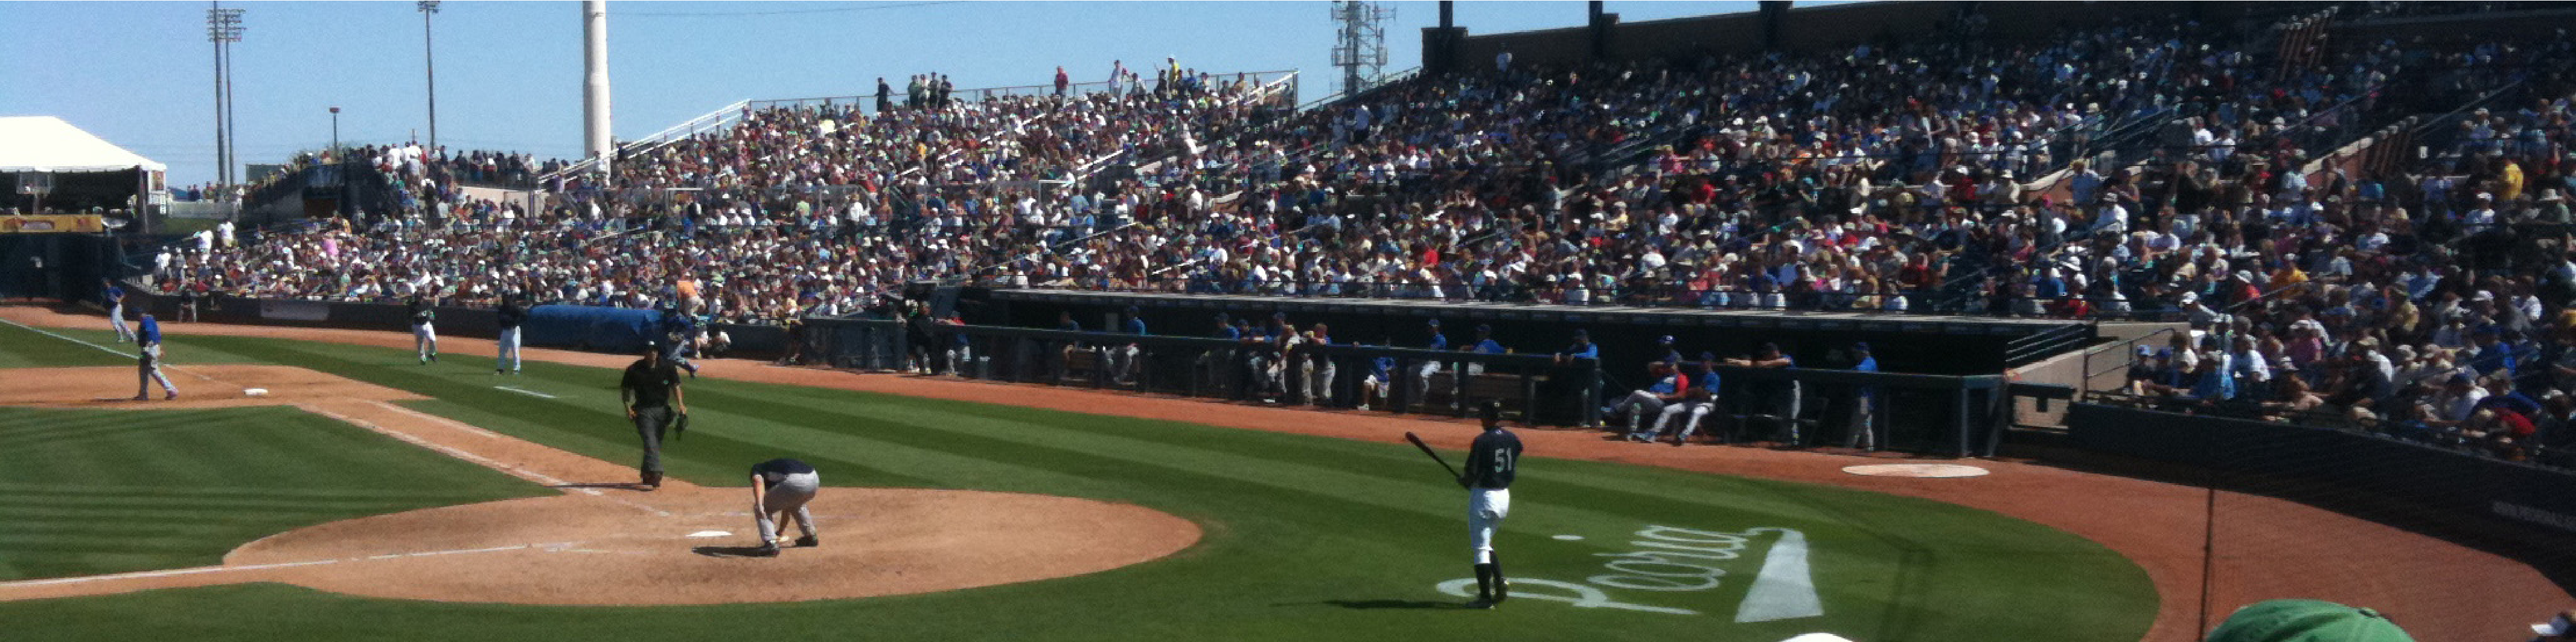
\includegraphics[width=\textwidth]{sampleteaser}
%   \caption{Seattle Mariners at Spring Training, 2010.}
%   \Description{Enjoying the baseball game from the third-base
%   seats. Ichiro Suzuki preparing to bat.}
%   \label{fig:teaser}
% \end{teaserfigure}

%%
%% This command processes the author and affiliation and title
%% information and builds the first part of the formatted document.
\maketitle

% 1
\section{Introduction}
\label{sec:introduction}
With the growing awareness of health management, wearable devices that record biometric information have become widely used. The recorded biometric information includes a variety of data, such as activity, respiration, body temperature, cardiac potential, blood pressure, gaze, pulse wave, and heart rate. The pulse sensor used to acquire the latter two kinds of data (i.e., the pulse wave and heart rate) irradiates the skin with LEDs that emit infrared light, red light, or green light with a wavelength around 550 nm. The oxidized hemoglobin in the blood flowing through arteries can absorb these lights. The pulse sensor takes advantage of the fact that the amount of reflected light decreases as the arterial blood flow increases with the timing of a heartbeat. Specifically, it uses a phototransistor to obtain changes in the amount of reflected light and measure the pulse wave. Here, the pulse wave data is numerical data on the changes in the reflected light, and the heart rate is measured by detecting the peaks that appear in the pulse wave data. This type of pulse wave measurement technique is called photoplethysmography (PPG) \cite{ppg}. Today's PPG sensors use the same principle as the device originally introduced by Hertzman \cite{ppg_principle1, ppg_principle2}, but in a smaller size using modern equipment. Many commercially available wearable devices (e.g., smartwatches) are equipped with a PPG sensor as a pulse sensor.\par

We speculate that it may be possible to measure an arbitrary pulse wave by inputting a change of light to a PPG sensor. Accordingly, we propose a method that enables a PPG sensor to acquire pulse data from a display. To simplify data collection for photoplethysmography imaging (PPGI), Paul et al. \cite{ppg_generator} developed a hardware PPG simulator by using an LED array to generate PPG signals. Our method differs in that it aims to use a small display device to input data to the PPG sensor of a wearable device. Specifically, our method inputs an arbitrary heart rate to a smartwatch. We set two objectives for the proposed method: PPG transfer and recognition of fake PPG data.\par

In terms of PPG transfer, artificial bodies and parts such as prosthetic hands, robotic arms, and telepresence robots do not have any blood flow, which makes it impossible to measure biometric data even if a smartwatch is worn on the wrist. While typical smartwatch functions such as calling, messaging, clocks, and payments, as well as sensors such as accelerometers and GPS sensors, can still be used with artificial limbs as with living limbs, pulse data cannot be measured. Meanwhile, when a smartwatch is attached to other body parts where blood flow exists (e.g., an ankle) to measure pulse data, the usability of other functions (e.g., messaging) is reduced. Other possible methods for PPG transfer include attachment of an additional PPG sensor to other body parts with blood flow and wireless input of the PPG data to the smartwatch, or detection of PPG data (or heart rate data) by non-PPG sensors \cite{heart_rate_accelerometer, Biowatch, SeismoTracker, heart_rate_ecg, heart_rate_touchscreen}. However, because most publicly available applications that use PPG data read the data from PPG sensors included in a device, the PPG data collected by these methods may not be usable for many applications.\par

In contrast, with the proposed method, even when a smartwatch is attached to an artificial limb, the user's pulse data can be read by changing the light of the display under the smartwatch's PPG sensor in accordance with pulse data measured at the junction of the living and artificial limbs. It is thus possible to use the normal functions of the smartwatch, because it is not modified and only the display is mounted on the artificial limb. Accordingly, users can still compare various aspects of commercial smartwatches, such as the design, function, and weight, and use the model of their choice. In addition, the smartwatch's PPG sensor can acquire data without modification of the smartwatch, which allows the user to still use common applications. Furthermore, in the case of a remote robot avatar, the operator's biometric data can be measured on the avatar's body.\par

As for recognition of fake PPG data, if a PPG sensor measures an arbitrary heart rate by the proposed method, it might be possible for a malicious user to falsify the heart rate and pretend to be exercising or continuing to rest. If a device using the proposed method becomes widely feasible and has a significant social impact, it will be necessary to examine the use of current PPG sensors in terms of this vulnerability.\par

In the rest of the paper, we introduce related works in Section \ref{sec:related}. We then explain the details of the proposed method in Section \ref{sec:method} and evaluate it in Section \ref{sec:evaluation}. Finally, Section \ref{sec:limitation} describes our method's limitations, and Section \ref{sec:conclusion} concludes the paper.



% 2
\section{Related Work}
\label{sec:related}
In this section, we introduce research on sensing with wearable devices, the use of smartwatches, and the use of pulse data.

% 2.1
\subsection{Sensing with Wearable Devices}
There is much research on wearable devices that are worn on body parts, and devices of various shapes have been investigated. Ham et al. \cite{smart_wristband} proposed a wristband-type device as an input device for smart glasses. The device is equipped with a touch panel and an inertial measurement unit, and it can be operated by touch or with a motion such as a twist of the wrist. Because the device is simply worn on the wrist, it offers a high degree of freedom by not restricting the user's movement. A touch panel is used for pointing to improve the input stability. Hernandez et al. \cite{bioglass} proposed a method for acquiring the pulse rate and respiration rate from data obtained from the accelerometer, gyroscope, and camera built into Google Glass, a head-mounted wearable device. Nishajith et al. \cite{smart_cap} designed and implemented ``Smart Cap,'' a wearable device to assist the visually impaired with situational awareness. The device consists of a Raspberry Pi 3, a Raspberry Pi NoIR Camera v2 (an infrared camera module for the Raspberry Pi), an earphone, and a power supply. The infrared camera obtains an image, and the object detected in the image is described by voice through the earphone.\par

For a non-optical approach, Bello et al. \cite{MoCapaci} proposed a wearable system that detects body postures and gestures without requiring sensors to be firmly fixed to the body or integrated into a tight-fitting garment. They implemented a prototype, ``MoCaBlazer,'' by using a standard men's blazer, and they conducted evaluation experiments with 14 subjects. For recognition of 20 actions, the system achieved average recognition accuracy of 97.18\% for leave-one-recording-out evaluation and 86.25\% for user-independent recognition.\par

Among research on other sensor modalities, Vargas et al. \cite{Brainwear} developed an open-source electroencephalography (EEG) sensing module with a state-of-the-art analog front end that is pin- and protocol-compatible with popular ecosystems in the wearable and DIY communities. The goal was to facilitate broad use of EEG sensing in multimodal smart garments. They conducted an evaluation experiment with a proof-of-concept application of the system in a normal baseball cap. They concluded that the system achieved similar levels of recognition to those in other neuroscience studies with dedicated instruments. R\"{o}ddiger et al. \cite{earables} conducted a study with seven different commercially available ``earables'' that are targeted at daytime usage: to investigate their comfort and wearability during sleep, they were all worn by 14 study participants. The results showed that devices occupying more space in the outer ear canal with rigid parts are less desirable. Vekemans et al. \cite{MOTUS} implemented ``MOTUS,'' a prototype watch-back tactile display that conveys emotions, to explore the potential for emotional expression by applying tactile texture patterns to the wrist. A preliminary guessability study with the prototype showed agreement between the texture patterns and the users' interpretation of emotions. Zhou et al. \cite{CoRSA} developed ``CoRSA,'' a lightweight system that supplements existing sports apparel having cardiorespiratory monitoring capabilities with system-in-package (SiP) and system-on-chip (SoC) sensors, which are popular in the wearable computing community. Other studies have examined wearable devices based on rings \cite{wearable_ring1, wearable_ring2, TypingRing, ElectroRing}, belts \cite{wearable_belt1, SmartBelt, WaistonBeltX, wearable_belt2}, and masks \cite{wearable_mask1, wearable_mask2, SilentMask, Masquare}.\par

Various body parts have been investigated as locations for wearable devices, and researchers have sought to estimate the locations from sensor data. Vahdatpour et al. \cite{localization_vahdatpour} collected acceleration data during daily activities from 25 subjects who wore accelerometers at 10 locations on the forearm, upper arm, head, thigh, shin, and waist. From the collected data, a support vector machine (SVM) was able to estimate the attachment site with an average accuracy of 89\%. Sztyler et al. \cite{localization_sztyler} collected acceleration data during various physical activities from 15 subjects who had accelerometers attached to seven locations: the head, chest, left upper arm, left wrist, waist, left pants pocket, and left ankle. From the collected data, the attachment site was estimated with an average accuracy of 89\% by using a random forest. Kunze et al. \cite{localization_kunze} collected data during walking movements from six subjects who had accelerometers attached to four locations: the wrist, the right side of the head above the eye, the left pants pocket, and the left breast pocket. From the collected data, the attachment site was estimated using the C4.5 classifier. In addition, we previously proposed a method to estimate the body part where a wearable device is attached without requiring the wearer to perform a specific action; instead, we used electrocardiography (ECG) and pulse data, which are biometric information that can be acquired by the wearable device \cite{localization_yoshida}.


% 2.2
\subsection{Studies on Smartwatches}
Among wearable devices, smartwatches have long been commercially available, and there is much research on them. Spinsante et al. \cite{accuracy_in_low_intensity} studied the heart rate obtained from a smartwatch during low-intensity physical activity and measured its accuracy. Sen et al. \cite{eating_recognition} proposed a method to record a user's eating behavior, such as the use of hands, chopsticks, or a spoon, by using data obtained from a smartwatch's accelerometer and gyroscope. By capturing food images with the smartwatch's built-in camera and performing image identification, the meal contents were also recorded. In another study, by leveraging the fact that smartwatches are always worn at the same location and in the same direction, Johnston et al. \cite{smartwatch_walk_authentication} proposed a method for biometric authentication based on gait data obtained from a smartwatch's accelerometer and gyroscope.\par

Smartphones are typically carried in a pants pocket or handbag, but compared to those locations, more activity information tends to be available at the wrist, where smartwatches are worn. Weiss et al. \cite{smartwatch_activity_recognition} showed that a smartwatch can identify actions more effectively than a smartphone in hand-based physical behaviors such as eating. The smartwatch could identify the behavior of ``drinking'' with 93.3\% accuracy, while the smartphone could only achieve 77.3\% accuracy.\par

Among other potential applications, Iakovakis et al. \cite{oh_detection} conducted a study on using a smartwatch to predict blood pressure drops due to postural changes. Orthostatic hypotension (OH) has been shown to cause dizziness and fainting and is a risk factor for falls in the young as well as the elderly. Accordingly, they proposed a mathematical prediction model that can reduce the risk of falls due to OH by sensing heart rate variability. Mauldin et al. \cite{smartfall} proposed an Android application, ``SmartFall,'' that detects falls by using acceleration data obtained from a commercially available smartwatch. The smartwatch is paired with a smartphone that runs the software. SmartFall communicates with a cloud server to perform the calculations necessary to predict falls in real time, while maintaining data privacy. Ciabattoni et al. \cite{smartwatch_stress_detection} proposed a method for detecting mental stress during various cognitive tasks in real time. Stress is classified by using galvanic skin response (GSR), RR interval (i.e., the time between successive R-peaks in an ECG), and body temperature data acquired by a commercial smartwatch. Sun et al. \cite{SleepMonitor} developed ``SleepMonitor,'' a smartwatch-based system for monitoring the user's respiratory rate and body position. The system uses accelerometer data collected at the wrist to estimate the respiratory rate. The results of evaluation experiments showed that the system could monitor the respiratory rate and body position during sleep with high accuracy under various conditions.\par

On the other hand, for an artificial limb, wearable devices cannot collect biometric information. In that case, methods using sensors such as accelerometers and gyroscopes are applicable, but methods using biometric data are not. Accordingly, we seek to make these applications available to users with artificial limbs as well as living limbs by inputting suitable data to the biometric sensors of wearable devices.


% 2.3
\subsection{Studies on Pulse Data}
Havriushenko et al. \cite{respiratory_rate_estimation1} proposed a method for estimating a user's respiratory rate from pulse wave data by using neural networks. The respiratory rate is often measured with a thermal sensor placed in the nasal channels or an elastic chest belt, but these devices may interfere with sleep. In contrast, their method can be implemented in a wearable device. The results of their evaluation showed an average respiratory rate estimation error lower than 2.2 breaths per minute. Jarchi et al. \cite{respiratory_rate_estimation2} proposed a method that relies on a nonlinear time-frequency representation, called the wavelet synchrosqueezed transform (WSST), to estimate the instantaneous respiratory rate from body-mounted PPG sensors. Han et al. \cite{arrhythmia_detection} proposed a method for detecting premature atrial contraction and premature ventricular contraction by using PPG data acquired from a smartwatch. Wang et al. \cite{alcohol_detection} developed a system for identifying excess alcohol consumption by using an SVM with data from ECG and PPG monitoring. Longmore et al. \cite{ppg_location} sought to identify a single location in the human anatomy for measuring simultaneously the heart rate (HR), blood oxygen saturation (SpO2), and respiration rate at rest and while walking by a single PPG sensor. In addition, we previously proposed a method to recognize the arm's muscle activity state and a method to estimate a surface electromyogram (sEMG) from PPG data \cite{semg_okamoto}. The results of an evaluation experiment with five participants showed that three types of muscle activity were recognized with over 75\% accuracy, and the sEMG was estimated with an error of approximately 20\%.\par

Among potential pulse data applications related to emotions, Goshvarpour et al. \cite{emotion_recognition1} proposed a method for classifying emotional responses by means of a simple dynamic signal processing technique and a fusion framework. They recorded the ECG and finger pulse activity of 35 subjects during a rest condition and when the subjects were listening to music that was intended to stimulate certain emotions. After constructing Poincar\'e plots, an SVM was used to classify them into four emotions: happiness, sadness, peacefulness, and fear. Kajiwara et al. \cite{emotion_recognition2} developed an application for logistics companies that adopt a manual order picking system, given that emotions and engagement affect work efficiency and human errors. Specifically, they proposed a method for predicting emotions and engagement during work with a high exercise intensity from behavior and pulse wave data acquired by wearable devices. Pulse wave, eye movement, and general movement data are input to deep neural networks to estimate a worker's emotion and engagement. The results of verification experiments showed that the emotion and engagement during order picking could be accurately predicted from the worker's behavior with an error rate of 0.12 or less. Lee et al. \cite{emotion_recognition3} conducted research on improving the speed of emotion recognition by using a PPG signal. A two-dimensional emotion model based on valence and arousal was adopted, and a one-dimensional convolutional neural network (1D CNN) was used to recognize emotions from a 1.1-s PPG signal. The 1D CNN was tested as a binary classifier (high or low valence and arousal) by using the dataset for emotion analysis using physiological signals (DEAP), and it achieved recognition accuracies of 75.3\% for valence and 76.2\% for arousal. Udovi\v{c}i\'{c} et al. \cite{emotion_recognition4} studied emotion recognition using only GSR and PPG signals because of their suitability for implementation in a simple wearable device that can collect signals from a person without compromising comfort and privacy. In addition to the above studies, there have been many others on the use of PPG data for emotion recognition \cite{emotion_recognition5, emotion_recognition6, emotion_recognition7}.\par

Pulse data is one of the most important pieces of biological information, as it can be applied to detect abnormalities in the body and recognize emotions. Most pulse sensors in commercially available wearable devices use PPG. As a result, when a wearable device is mounted on an artificial limb, where there is no blood flow, pulse data cannot be acquired. Hence, among various kinds of biometric data, we focus on pulse data and propose a method to allow a wearable device to measure pulse data similar to that of a living limb even on an artificial limb.



% 3
\section{Proposed Method}
\label{sec:method}

% 3.1
\subsection{Overview}
In our proposed method, when a user sets an arbitrary heart rate, a display lights up, and a smartwatch worn over the display measures the specified heart rate. \figref{method} illustrates the process flow of the proposed method. First, the user's real (target) heart rate is obtained by a PPG sensor that is separate from the smartwatch. Next, the brightness of the display, which is connected to a microcomputer, is changed according to the target heart rate. Finally, the smartwatch measures the heart rate indicated by the display, which is the same as the target heart rate.

\begin{figure}[!t]
  \centering
  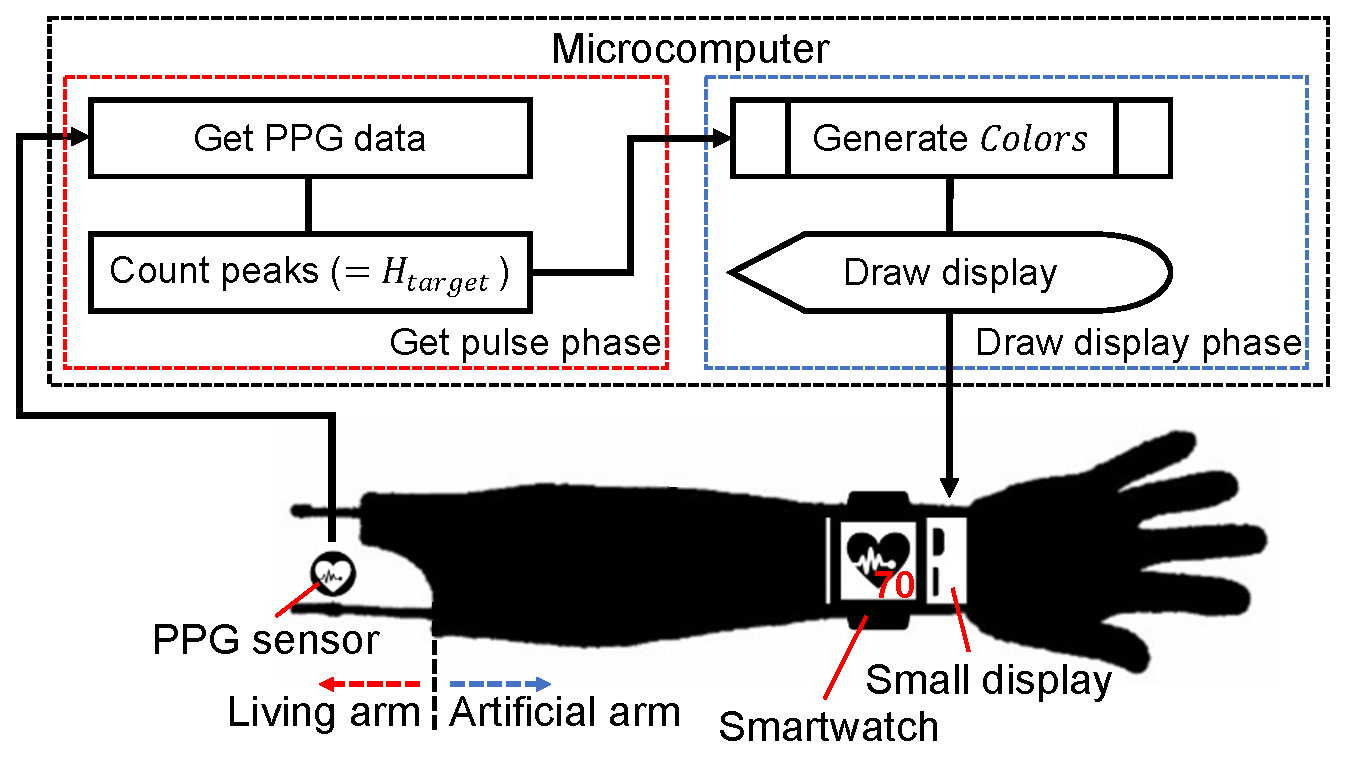
\includegraphics[width=1\linewidth]{figures/method.eps}
  \caption{Process flow of the proposed method.}
  \label{fig:method}
\end{figure}


% 3.2
\subsection{Target Heart Rate Calculation}
We denote the target heart, which is determined from the wearer's heart rate, as $H_{target}$. It is computed from two thresholds, $Threshold_{value}$ and $Threshold_{time}$, by using the PPG sensor, which constantly measures data. By using this data, the system records the times of pulse peak occurrences. A peak is detected when the PPG data measured in real time exceeds $Threshold_{value}$, but not until more than $Threshold_{time}$ time has passed since the last peak occurred. In this work, $Threshold_{value}$ and $Threshold_{time}$ were heuristically set to 700 and 0.3, respectively; in practice, however, they should be adjusted according to the environment in which the system is used. When a peak is detected, the time difference from the previous peak occurrence time is calculated. Here, the time difference refers to the RR interval, denoted as $RR$ [s], which is the time between one ventricular activation and the next. The number of times the ventricles contract in one minute is the heart rate in beats per minute (bpm). Therefore, if the RR interval is known, the heart rate $H_{target}$ can be calculated by the following equation:
\begin{equation}
  \label{eqn:target}
  H_{target} = int(60 / RR).
\end{equation}
The system continuously updates this value.\par

$H_{target}$ can also be set manually if the user wants the smartwatch to measure a specific heart rate. \figref{system} shows a system implementation in which the target heart rate is manually set from a control application and the heart rate is input to the smartwatch on an artificial arm.

\begin{figure}[!t]
  \centering
  \includegraphics[width=1\linewidth]{figures/system.eps}
  \caption{System implementation in which the target heart rate is manually set from a control application and the heart rate is input to the smartwatch on an artificial arm.}
  \label{fig:system}
\end{figure}


% 3.3
\subsection{Display Control}
Next, the display's brightness is controlled so that the heart rate measured by the smartwatch matches $H_{target}$. An array, denoted as $Colors$, is prepared in advance to store the required brightness for the smartwatch to detect a single pulse peak.\par

PPG sensors use LEDs to irradiate infrared, red, or green light onto the skin and measure pulse data from changes in the light reflected from the blood vessels. Because blood flow increases with the timing of the pulse, the blood vessels absorb more light, and the reflected light becomes dimmer. Because black absorbs more light than white, as the display is rendered blacker, the light emitted from the smartwatch and reflected by the display becomes darker.\par

Hence, the proposed method draws the values in $Colors$ on the display one by one during each drawing interval $T$ [s]. We set $T$ for each value in $Colors$ as follows, so that $Colors$ is applied $H_{target}$ times in one minute:
\begin{equation}
  \label{eqn:wait}
  T = 60 / \{len(Colors) * H_{target}\},
\end{equation}
where $len(Colors)$ is the data length of $Colors$.


% 3.4
\subsection{Pulse Data Measurement}
Finally, in the proposed method, pulse data is measured by the smartwatch worn over the blinking display. Such pulse data measured by a PPG sensor on a smartwatch can be used in various applications. However, the performance of the PPG sensor and the algorithm for measuring pulse data vary among different smartwatch models and are not publicly accessible. Accordingly, we manually set the target heart rate in our evaluation experiment described below.



% 4
\section{Evaluation}
\label{sec:evaluation}
This section describes experiments that we conducted to evaluate the effectiveness of the proposed method. Specifically, we evaluated the heart rate acquired by a smartwatch when an arbitrary target heart rate was given. We then observed the error between the target heart rate and the heart rate obtained by the smartwatch and investigated the effects of various smartwatches and displays.

% 4.1
\subsection{Evaluation Environment}
We used five smartwatches for the evaluation experiment: the TicWatch Pro WF12106, Puma Smartwatch PT9100, Apple Watch Series 3 and Series 5, and SMART R F-18. We also used four different displays: the display of the Lenovo Legion 7 15IMH05 laptop (display A); two 3.5-inch displays developed for Raspberry Pi by Elecrow and Osoyoo (displays B and C, respectively); and a lightweight flexible display \cite{flexible_display} that we constructed (display D). \figref{smartwatches} shows all the smartwatches and displays that we used, and \figref{flexible} shows the details of display D.

\begin{figure}[!t]
  \centering
  \includegraphics[width=1\linewidth]{figures/smartwatches.eps}
  \caption{Smartwatches and displays used in the experiment.}
  \label{fig:smartwatches}
\end{figure}

\begin{figure}[!t]
  \centering
  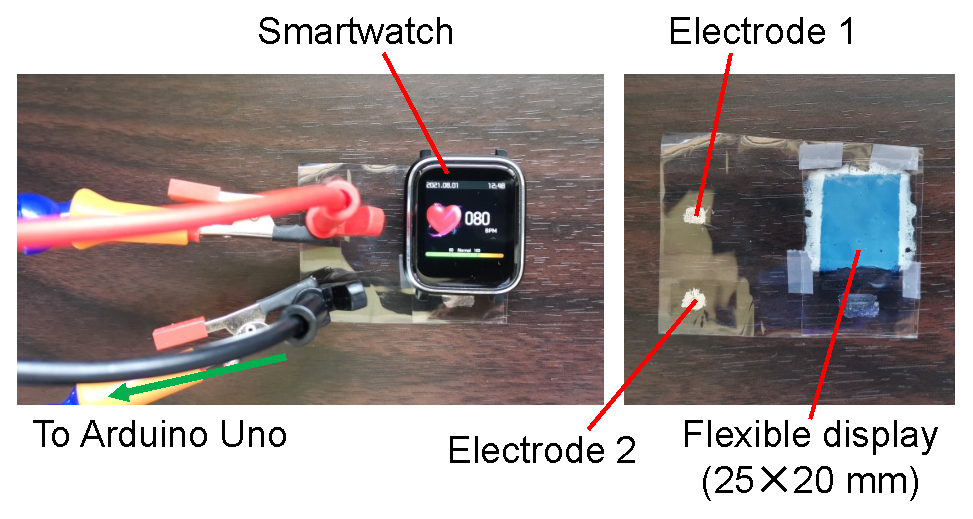
\includegraphics[width=1\linewidth]{figures/flexible.eps}
  \caption{Illustration of the flexible display (display D).}
  \label{fig:flexible}
\end{figure}


% 4.2
\subsection{Display Drawing Program Implementations}
The four displays used in the evaluation experiment had different connection methods to the computer. Display A was a laptop display, and commercial displays B and C could use an HDMI connection. In contrast, display D required drawing on the screen by controlling the voltage applied to the display's electrodes. In this section, we explain the display drawing programs that we implemented to control each display.

% 4.2.1
\subsubsection{Displays A, B, and C}
Displays A, B, and C were all recognized by the computer as regular displays. The $Colors$ data was represented in grayscale, a type of computer color representation that uses 256 levels (0--255) to represent shades of color from black to white (i.e., smaller values represent darker shades). Each array element $Colors[i]~(i=0,\dots,L)$ was generated by the following equation:
\begin{equation}
  Colors[i]=\min\left(\sin\left(\frac{2\pi i}{L}\right)+1,1\right)*SCALE+BASE,
\end{equation}
where the values of $L$, $SCALE$, and $BASE$ were heuristically determined in advance for each display-smartwatch combination.\par

For example, if $L=19$, $SCALE=30$, and $BASE=225$, then $Colors$ was obtained as the following sequence of numbers:
\begin{equation*}
  \begin{split}
    Colors = [255, 255, 255, 255, 255, 255, 255, 255, 255, 255,\\250, 240, 232, 227, 225, 225, 229, 236, 245, 255]
  \end{split}
\end{equation*}
\figref{colors_wave} shows a plot of this particular $Colors$ array.\par

A program to change the brightness of displays A, B, and C was implemented with Python and Processing. Processing\footnote{\url{https://processing.org}} is a Java-based programming language that is excellent for visual expression and is used to create electronic art and visual designs. Here, the Processing component receives the target heart rate from the Python component, and it uses the \texttt{background} method to draw the appropriate grayscale background color on the display.

\begin{figure}[!t]
  \centering
  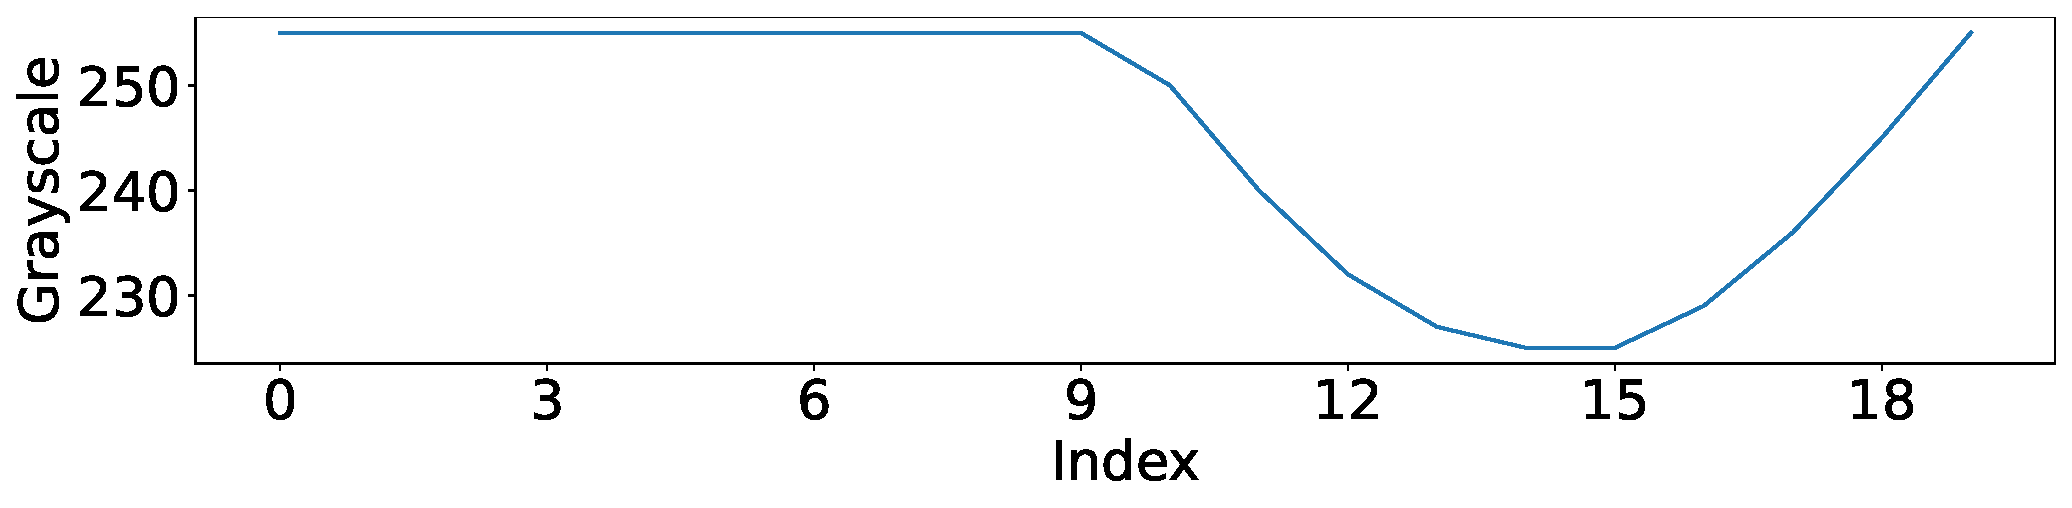
\includegraphics[width=1\linewidth]{figures/colors_wave.eps}
  \caption{Example plot of light and dark changes in the display for the smartwatch to detect a single pulse peak.}
  \label{fig:colors_wave}
\end{figure}

% 4.2.2
\subsubsection{Display D}
Display D was made of a flexible film that could fit on curved areas like an arm or the back of a smartwatch, but it did not have HDMI capability. Instead, it was made to blink by switching the potential direction applied to its terminals. The display color became darker when a higher voltage was applied to electrode 1 and lighter when a higher voltage was applied to electrode 2.\par

As a result of a heuristic search in a preliminary study, $Colors$ was determined to be the following sequence of colors for display D:
\begin{equation*}
  \begin{split}
    Colors = [BLACK, WHITE].
  \end{split}
\end{equation*}
For $BLACK$, we set the voltage of electrode 1 to 2 V and that of electrode 2 to 0 V; for $WHITE$, we set the voltage of electrode 1 to 0 V and that of electrode 2 to 2 V. \figref{colors_flexible} shows how the voltage changed when the pattern in $Colors$ was repeated twice.\par

For display D, we implemented a display drawing program by using the Arduino Uno R3 microcomputer, which could control the output voltage by pulse-width modulation (PWM). After receiving the target heart rate from the Python component running on a connected computer, the Arduino changed the voltage to the display.

\begin{figure}[!t]
  \centering
  \includegraphics[width=1\linewidth]{figures/voltage_wave.eps}
  \caption{Voltage changes when the pattern in $Colors$ was repeated twice.}
  \label{fig:colors_flexible}
\end{figure}


% 4.3
\subsection{Data Acquisition}
Depending on the installed operating system (OS), the five smartwatches had different ways of acquiring the heart rate. In this subsection, we describe how the heart rate was acquired for each OS.

% 4.3.1
\subsubsection{Wear OS}
The TicWatch Pro WF12106 and the Puma Smartwatch PT9100 both use Wear OS by Google\footnote{\url{https://wearos.google.com}}, an OS that was designed for smartwatches and is based on Android. We used Android Studio\footnote{\url{https://developer.android.com/studio}} to implement the control application, which is illustrated in \figref{app}.\par

When the application is started, it displays the screen shown in (1). Acquisition of the sensor value starts automatically, and when the value changes, it is displayed as shown in (2). ``Heart'' indicates the value from the heart rate sensor, and ``Pulse'' indicates the value from the PPG sensor. Data recording is begun by tapping the ``RECORD'' button. A 60-s calibration then starts as shown in (3). This calibration waits for the sensor value to stabilize, and the wearing position of the smartwatch can be adjusted during this period. When the 60-s calibration is complete, sensor data is acquired for 60 s as shown in (4) and stored in a variable. At the end of the data acquisition period, the data stored in the variable is saved to the smartwatch in CSV format, and a message indicating the completion of data acquisition is displayed as shown in (5). The smartwatch is equipped with a variety of sensors, and the data is accessed by specifying the sensor number during application development\footnote{\url{https://developer.android.com/reference/android/hardware/Sensor}} (e.g., sensor number 21 and 65572 for the heart rate sensor and the PPG sensor in this application). The rate of ``SENSOR\_DELAY\_UI'' events was used to set a sampling rate that was suitable for implementing the user interface\footnote{\url{https://developer.android.com/reference/android/hardware/SensorManager}}.\par

In the evaluation experiment, data acquisition was started by placing the smartwatch on the display, entering the target heart rate into the standard input of the display drawing program, and tapping the ``RECORD'' button in the smartwatch application. After 120 s, including the 60-s calibration, the data acquisition was complete. The sampling rate for heart rate data acquisition was approximately 1 Hz. As shown in \figref{calculating_heart_rate_wearos}, the time average of 60 s of data (excluding the calibration period) was calculated, and the result was obtained as the heart rate.

\begin{figure}[!t]
  \centering
  \includegraphics[width=1\linewidth]{figures/app.eps}
  \caption{Details of the control application implemented for the Wear OS smartwatches.}
  \label{fig:app}
\end{figure}

\begin{figure}[!t]
  \centering
  \begin{minipage}[t]{1\linewidth}
    \centering
    \includegraphics[width=1\linewidth]{figures/calculating_wearos.eps}
    \subcaption{Wear OS smartwatches}
    \small The time average of 60 s of data, excluding the 60 s of calibration time, was calculated as the heart rate result.
    \label{fig:calculating_wearos}
    \vspace{10pt}
  \end{minipage}
  \begin{minipage}[t]{1\linewidth}
    \centering
    \includegraphics[width=1\linewidth]{figures/calculating_watchos.eps}
    \subcaption{watchOS smartwatches}
    \small The first 30 s of data was excluded as calibration time, and the time average of the following 60 s of data was calculated as the heart rate result.
    \label{fig:calculating_watchos}
    \vspace{10pt}
  \end{minipage}
  \begin{minipage}[t]{1\linewidth}
    \centering
    \includegraphics[width=1\linewidth]{figures/calculating_originalos.eps}
    \subcaption{SMART OS smartwatch}
    \small The heart rate displayed in the app was recorded manually as the heart rate result.
    \label{fig:calculating_originalos}
  \end{minipage}
  \caption{Heart rate calculations for the smartwatches in the evaluation experiment.}
  \label{fig:calculating_heart_rate}
\end{figure}

% 4.3.2
\subsubsection{watchOS}
The Apple Watch Series 3 and Series 5 come standard with Apple's Heart Rate app that measures the heart rate\footnote{\url{https://support.apple.com/en-us/HT204666}}. The collected heart rate data can be output as numerical data in XML format by using the iPhone Health app when paired with the Apple Watch\footnote{\url{https://support.apple.com/guide/iphone/share-health-and-fitness-data-iph27f6325b2/ios}}.\par

In the evaluation experiment, data acquisition was started by placing the smartwatch on the display, entering the target heart rate into the standard input of the display drawing program, and launching the Heart Rate app. After a period of time, the Apple Watch display automatically turned off, and the data acquisition was complete. The data acquisition time was not configurable, but we found a maximum time of approximately 160 s. The sampling rate was not publicly accessible, and the amount of data acquired in a single data acquisition trial varied. As shown in \figref{calculating_heart_rate_watchos}, the first 30 s of data was excluded as calibration time, and the time average of the following 60 s of data was calculated as the result for the heart rate. However, when no data was acquired after the calibration time, the last acquired data was used as the heart rate.

% 4.3.3
\subsubsection{SMART OS}
The SMART R F-18 is equipped with a proprietary OS developed by the manufacturer, and we refer to it here as ``SMART OS.'' Heart rate data collected by this smartwatch can be viewed with the WearHealth app for Android\footnote{\url{https://play.google.com/store/apps/details?id=com.zjw.wearhealth}} and iPhone\footnote{\url{https://apps.apple.com/us/app/wearhealth/id1265052549}}.\par

In the evaluation experiment, data acquisition was started by placing the smartwatch on the display, entering the target heart rate into the standard input of the display drawing program, and controlling the smartwatch from the WearHealth app on the smartphone. After 30 s, the data acquisition was complete, and the resulting heart rate was displayed in the app. The sampling rate and the algorithm to determine the resulting heart rate were not publicly accessible for the SMART R F-18. As shown in \figref{calculating_heart_rate_originalos}, the heart rate result shown in the app was recorded manually.


% 4.4
\subsection{Results and Discussion}
To obtain the correct heart rate, an acrylic plate of a certain thickness was placed between the display and the smartwatch in some display-smartwatch combinations. \tabref{acrylic_plate} lists these combinations and the thicknesses of the acrylic plate, with a blank cell indicating that the plate was not used.\par

The error of the measured heart rate was calculated by subtracting the target heart rate from it. The target heart rate was tested at intervals of 5 bpm from 60 to 100 bpm, which is the resting heart rate range for adults\footnote{\url{https://www.heart.org/en/healthy-living/fitness/fitness-basics/target-heart-rates}}. \tabref{result} lists the results of the evaluation experiment, which were averaged over three sets of measurements. The results were rounded to the first decimal place. A zero means that the measured heart rate was the same as the target heart rate, and a negative value means that the measured heart rate was smaller. An $NaN$ entry indicates that the heart rate measurement failed.\par

In addition, \tabref{result_expansion} lists the results of a separate experiment using display D with target heart rates set of 40--55 bpm (heart rate during sleep) and 105--200 bpm (heart rate during exercise).

\begin{table*}[!t]
  \small
  \centering
  \caption{Thickness of the acrylic plate placed between the display and the smartwatch.}
  \begin{tabular}{cccc|cccc|cccc|cccc|cccc}
    \toprule
    \multicolumn{4}{c|}{TicWatch Pro}&\multicolumn{4}{c|}{Puma}&\multicolumn{4}{c|}{Series 3}&\multicolumn{4}{c|}{Series 5}&\multicolumn{4}{c}{SMART R} \\
    A & B & C & D & A & B & C & D & A & B & C & D & A & B & C & D & A & B & C & D \\
    \midrule
    -- & 2 mm & -- & 5 mm & -- & -- & -- & 2 mm & -- & -- & -- & -- & -- & 2 mm & -- & -- & 2 mm & -- & -- & -- \\
    \bottomrule
  \end{tabular}
  \label{tab:acrylic_plate}
\end{table*}

\begin{table*}[!t]
  \small
  \centering
  \caption{Error in the resting heart rate obtained by the TicWatch Pro, Puma Smartwatch, Apple Watch Series 3, Apple Watch Series 5, and SMART R (display A: Lenovo Legion 7; B: 3.5-inch Elecrow; C: 3.5-inch Osoyoo; D: flexible display).}
  \begin{tabular}{c|cccc|cccc}
    \toprule
    &\multicolumn{4}{c|}{TicWatch Pro}&\multicolumn{4}{c}{Puma} \\
    $H_{target}$ & A & B & C & D & A & B & C & D \\
    \midrule
    $60$ & $-1.7$ & $-1.4$ & $-1.4$ & $-2.0$ & $-1.7$ & $-1.4$ & $-1.4$ & $-0.8$ \\
    $65$ & $-1.8$ & $-1.4$ & $-1.3$ & $-2.5$ & $-1.8$ & $-1.4$ & $-1.3$ & $-1.8$ \\
    $70$ & $-1.8$ & $-2.1$ & $-1.2$ & $-0.4$ & $-1.8$ & $-2.1$ & $-1.2$ & $-0.9$ \\
    $75$ & $-2.2$ & $-1.6$ & $-1.5$ & $-0.1$ & $-2.2$ & $-1.6$ & $-1.5$ & $-1.2$ \\
    $80$ & $-2.0$ & $-1.5$ & $-1.1$ & $0.6$ & $-2.0$ & $-1.5$ & $-1.1$ & $0.0$ \\
    $85$ & $-1.8$ & $-1.5$ & $-1.6$ & $0.5$ & $-1.8$ & $-1.5$ & $-1.6$ & $0.3$ \\
    $90$ & $-2.0$ & $-1.7$ & $-1.0$ & $-0.4$ & $-2.0$ & $-1.7$ & $-1.0$ & $-0.5$ \\
    $95$ & $-2.0$ & $-1.2$ & $-1.1$ & $0.0$ & $-2.0$ & $-1.2$ & $-1.1$ & $-1.2$ \\
    $100$ & $-1.9$ & $-1.5$ & $-1.4$ & $-1.0$ & $-1.9$ & $-1.5$ & $-1.4$ & $-1.2$ \\
    \midrule
    Average & $-1.9$ & $-1.5$ & $-1.3$ & $-0.6$ & $-1.9$ & $-1.5$ & $-1.3$ & $-0.8$ \\
    \bottomrule
  \end{tabular}
  \begin{tabular}{c|cccc|cccc|cccc}
    \toprule
    &\multicolumn{4}{c|}{Series 3}&\multicolumn{4}{c|}{Series 5}&\multicolumn{4}{c}{SMART R} \\
    $H_{target}$ & A & B & C & D & A & B & C & D & A & B & C & D \\
    \midrule
    $60$ & $0.4$ & $1.0$ & $-0.2$ & $NaN$ & $58.2$ & $0.1$ & $-0.1$ & $0.0$ & $-1.7$ & $-1.0$ & $-1.7$ & $-0.7$ \\
    $65$ & $0.6$ & $0.1$ & $-0.1$ & $NaN$ & $16.1$ & $-0.4$ & $0.1$ & $0.0$ & $-1.7$ & $-1.0$ & $-0.7$ & $-0.7$ \\
    $70$ & $0.1$ & $2.0$ & $0.0$ & $NaN$ & $1.6$ & $2.4$ & $0.1$ & $0.0$ & $-1.0$ & $-1.3$ & $-1.3$ & $-0.7$ \\
    $75$ & $0.0$ & $2.8$ & $-0.6$ & $NaN$ & $0.8$ & $0.1$ & $-0.2$ & $-0.1$ & $-2.0$ & $-2.3$ & $-2.0$ & $-0.7$ \\
    $80$ & $-0.5$ & $1.0$ & $-0.5$ & $NaN$ & $1.2$ & $0.9$ & $-0.4$ & $-0.5$ & $-2.0$ & $-2.0$ & $-1.0$ & $-1.0$ \\
    $85$ & $-5.4$ & $-0.7$ & $-0.6$ & $NaN$ & $-0.6$ & $-1.0$ & $-0.9$ & $0.0$ & $-2.0$ & $-2.0$ & $-1.7$ & $-0.7$ \\
    $90$ & $-0.6$ & $-1.3$ & $-0.6$ & $NaN$ & $4.3$ & $-1.0$ & $-0.9$ & $0.0$ & $-3.3$ & $-2.3$ & $-1.7$ & $-1.0$ \\
    $95$ & $-1.5$ & $-0.5$ & $-1.0$ & $NaN$ & $-0.1$ & $-0.3$ & $-1.1$ & $0.0$ & $-2.7$ & $-2.0$ & $-2.0$ & $-0.3$ \\
    $100$ & $-0.7$ & $-1.1$ & $-0.7$ & $NaN$ & $-0.2$ & $-7.3$ & $-0.8$ & $-32.7$ & $-2.7$ & $-2.3$ & $-2.7$ & $-1.0$ \\
    \midrule
    Average & $-0.8$ & $0.4$ & $-0.5$ & $NaN$ & $9.0$ & $-0.7$ & $-0.5$ & $-3.7$ & $-2.1$ & $-1.8$ & $-1.6$ & $-0.7$ \\
    \bottomrule
  \end{tabular}
  \label{tab:result}
\end{table*}

\begin{table*}[!t]
  \small
  \centering
  \caption{Error in the heart rate during sleep or exercise obtained by the TicWatch Pro, Puma Smartwatch, Apple Watch Series 3, Apple Watch Series 5, and SMART R with display D (the flexible display).}
  \begin{tabular}{c|c|c|c|c|c}
    \toprule
    & TicWatch Pro & Puma & Series 3 & Series 5 & SMART R \\
    $H_{target}$ & D & D & D & D & D \\
    \midrule
    $40$ & $0.0$ & $0.0$ & $NaN$ & $3.1$ & $23.7$ \\
    $45$ & $-1.2$ & $-1.0$ & $NaN$ & $0.1$ & $31.7$ \\
    $50$ & $-1.7$ & $-0.8$ & $NaN$ & $0.0$ & $0.3$ \\
    $55$ & $-0.7$ & $-0.7$ & $NaN$ & $0.0$ & $0.0$ \\
    \vdots & \vdots & \vdots & \vdots & \vdots & \vdots \\
    $105$ & $-0.2$ & $0.0$ & $NaN$ & $-34.3$ & $0.0$ \\
    $110$ & $-0.2$ & $0.0$ & $NaN$ & $-0.2$ & $-0.3$ \\
    $115$ & $-0.2$ & $0.3$ & $NaN$ & $-39.3$ & $-0.3$ \\
    $120$ & $-0.3$ & $-0.7$ & $NaN$ & $-41.5$ & $-0.7$ \\
    $125$ & $-0.8$ & $0.0$ & $NaN$ & $-0.7$ & $-0.3$ \\
    $130$ & $0.9$ & $0.3$ & $NaN$ & $-41.9$ & $0.0$ \\
    $135$ & $0.0$ & $-0.8$ & $NaN$ & $-41.7$ & $-0.3$ \\
    $140$ & $0.2$ & $-0.3$ & $NaN$ & $-70.7$ & $0.0$ \\
    $145$ & $0.7$ & $-0.2$ & $NaN$ & $-40.2$ & $0.3$ \\
    $150$ & $-0.1$ & $-0.3$ & $NaN$ & $-0.6$ & $-0.3$ \\
    $155$ & $0.5$ & $0.0$ & $NaN$ & $0.1$ & $0.0$ \\
    $160$ & $0.6$ & $0.0$ & $NaN$ & $0.0$ & $-0.3$ \\
    $165$ & $1.7$ & $1.3$ & $NaN$ & $0.0$ & $0.7$ \\
    $170$ & $0.0$ & $0.7$ & $NaN$ & $-94.4$ & $0.0$ \\
    $175$ & $0.3$ & $0.0$ & $NaN$ & $-50.6$ & $-0.7$ \\
    $180$ & $0.3$ & $0.6$ & $NaN$ & $-63.0$ & $0.0$ \\
    $185$ & $1.0$ & $-0.4$ & $NaN$ & $-0.3$ & $0.3$ \\
    $190$ & $1.4$ & $-0.2$ & $NaN$ & $-86.8$ & $0.3$ \\
    $195$ & $0.3$ & $1.7$ & $NaN$ & $-83.4$ & $0.3$ \\
    $200$ & $0.6$ & $0.0$ & $NaN$ & $-103.0$ & $0.0$ \\
    \bottomrule
  \end{tabular}
  \label{tab:result_expansion}
\end{table*}

% 4.4.1
\subsubsection{Wear OS Smartwatches}
The results showed that the heart rate could be input to the smartwatch within an error of less than $3$ bpm. For both Wear OS smartwatches, the average error was progressively smaller for displays A, B, C, and D, in that order. This suggests that differences in performance, such as the display brightness and refresh rate, may affect the generated heart rate. As seen in \tabref{result_expansion}, even when the target heart rate was set to 40--55 or 105--200 bpm, the heart rate could be input to the smartwatch within a small error.

% 4.4.2
\subsubsection{watchOS Smartwatches}
The results showed that display C enabled the heart rate to be input to the Apple Watches within an error of $-1.1$ to $0.1$ bpm. On the other hand, with displays A and B, we could not obtain the correct heart rate under certain conditions. In particular, the correct heart rate was not obtained even once with a target heart rate of 60 bpm and the combination of the Apple Watch Series 5 and display A.\par

When the target heart rate was set to 40--55 and 105--200 bpm, correct values were obtained for some target heart rates with the Apple Watch Series 5. When the target heart rate was set above 100 bpm, the obtained rate was very small compared to the target rate. It is possible that the Apple Watch algorithm recognized large target heart rates as incorrect and calibrated them to the heart rates during rest.\par

The combination of the Apple Watch Series 3 and display D failed to measure the heart rate regardless of the target. Because a PPG sensor uses a photoreflector, it is easily affected by light, and depending on the condition of the wearable device's placement, pulse data cannot always be acquired correctly. Whether a smartwatch can recognize a generated pulse wave is thought to depend on the shape of the device's PPG sensor. The acrylic plates that we used in this paper could not help the performance of the Apple Watch Series 3, but it is possible that pulse data could be successfully recognized by using a plate with a different material and thickness.

% 4.4.3
\subsubsection{SMART OS Smartwatch}
Finally, the results showed that the heart rate could almost always be input to this smartwatch within an error of less than $3$ bpm. With display D, in particular, it could be obtained within an error of less than $1$ bpm.\par

When the target heart rate was set to 40--55 and 105--200 bpm, the heart rate could be input to the smartwatch with a very small error in many cases; for target rates below 50 bpm, however, the heart rate could not be input correctly. This is thought to be due to a performance limitation of the smartwatch's PPG sensor.



% 5
\section{Limitations}
\label{sec:limitation}
The results in Section \ref{sec:evaluation} showed that the measured heart rate could be input to the smartwatch with small errors in most cases. This section discusses the limitations of the proposed method in terms of other pulse-wave-related indices and the pulse waveform.\par

For comparison, we acquired real raw PPG data from the main author's left index finger and raw PPG data generated by display D with a 2-mm acrylic plate. \figref{raw_data_acquisition} illustrates the environment during this raw pulse data acquisition. Numerical pulse data was collected at a sampling rate of 106 Hz for 60 s by using an Arduino Uno R3 and a PPG sensor\footnote{\url{https://www.pulsesensor.com}}. The Arduino used here was different from the one used to control the display.

\begin{figure}[!t]
  \centering
  \includegraphics[width=1\linewidth]{figures/raw_data_acquisition.eps}
  \caption{Environment during raw pulse data acquisition.}
  \label{fig:raw_data_acquisition}
\end{figure}


% 5.1
\subsection{Pulse Wave Status Indicators}
The raw PPG data was analyzed using Kubios HRV Premium (ver. 3.5.0)\footnote{\url{https://www.kubios.com/hrv-premium}}, a fully featured heart rate variability (HRV) analysis software package. \figref{rr_wave} shows the resulting RR time series data, \tabref{report_real} lists the analysis results for the real PPG data, and \tabref{report_generated} lists the results for the generated PPG data. The values in these analysis results were calculated from the RR time series data. The target heart rate at the time of pulse wave generation was set to 68 bpm, which was the mean heart rate (HR) of the real pulse wave obtained from the finger.\par

The results showed that the generated pulse wave was at 68 bpm for both the minimum HR and the maximum HR. They also showed that the target heart rate could be input to the PPG sensor in a stable manner, as in the main experiment described in Section \ref{sec:evaluation}. As for the RR interval, it is regular under normal conditions but generally varies during relaxation, when the heart is less active. In these results, the mean RR was normal and close between the real and generated pulse waves, which indicates that the generated pulse wave could be recognized as a correct pulse waveform. The standard deviation of the RR interval, denoted as SDNN, was very small for the generated pulse wave. The reason might be that, because the mechanically generated pulse wave was a stable waveform, there was no variation in the RR intervals; this was confirmed by the results shown in \figref{rr_wave}.\par

In pulse wave data, the low-frequency power (LF) indicates both sympathetic and parasympathetic nervous system activity, while the high-frequency power (HF), also known as respiratory sinus arrhythmia (RSA), indicates parasympathetic activity and variation of the RR intervals with respiration. The heart rate increases with inhalation and decreases with exhalation. Because LF appears regardless of whether the sympathetic or parasympathetic nervous system is dominant, the ratio of LF to HF (LF/HF ratio) is used as a stress indicator. In a relaxed state, the parasympathetic nervous system is activated, which results in HF indicating respiratory variations and LF indicating blood pressure variations. On the other hand, under stressful conditions, the sympathetic nervous system is activated, and LF still appears but HF decreases. Therefore, HF is relatively larger in a relaxed state, so the LF/HF ratio is small, while LF is relatively larger in a stressed state, so the LF/HF ratio is large. However, the criterion of the LF/HF ratio for judging stressful conditions depends on individual differences and the measurement conditions. The results here for the power (\%) and the LF/HF ratio of the generated pulse wave showed that HF was large, which indicated a relaxed state. However, this result was inconsistent with the small variation in the RR interval. Because the generated PPG data was not intended to control LF and HF, these values merely resulted from the frequency analysis of the RR interval data, and they may be meaningless. If we can generate more detailed PPG data in the future, it may become possible to control the LF/HF ratio.

\begin{figure*}[!t]
  \centering
  \includegraphics[width=1\linewidth]{figures/rr_wave.eps}
  \caption{RR time series data.}
  \label{fig:rr_wave}
\end{figure*}

\begin{table*}[!t]
  \small
  \centering
  \caption{Analysis results for the real PPG data.}
  \begin{minipage}[t]{0.45\linewidth}
    \centering
    \subcaption{Time-Domain Results}
    \begin{tabular}{lrr}
    \toprule
    Variable & Units & Value \\
    \midrule
    Mean RR & (ms) & $887$ \\
    Mean HR & (bpm) & $68$ \\
    Min HR & (bpm) & $63$ \\
    Max HR & (bpm) & $74$ \\
    SDNN & (ms) & $37.5$ \\
    RMSSD & (ms) & $49.4$ \\
    NN50 & (beats) & $20$ \\
    pNN50 & (\%) & $33.90$ \\
    RR triangular index & & $7.50$ \\
    TINN & (ms) & $149.0$ \\
    Stress Index (SI) & & $12.8$ \\
    DC & (ms) & $26.6$ \\
    DCmod & (ms) & $51.4$ \\
    \bottomrule
    \end{tabular}
  \end{minipage}
  \begin{minipage}[t]{0.45\linewidth}
    \centering
    \subcaption{Frequency-Domain Results (FFT spectrum)}
    \begin{tabular}{lrrrr}
    \toprule
    Variable & Units & VLF & LF & HF \\
    \midrule
    Frequency band & (Hz) & $0.00\text{--}0.04$ & $0.04\text{--}0.15$ & $0.15\text{--}0.40$ \\
    Peak frequency & (Hz) & $0.040$ & $0.113$ & $0.350$ \\
    Power & (ms${}^\text{2}$) & $113$ & $800$ & $657$ \\
    Power & (log) & $4.726$ & $6.684$ & $6.488$ \\
    Power & (\%) & $7.17$ & $50.84$ & $41.79$ \\
    Power & (n.u.) & & $54.77$ & $45.02$ \\
    \text{-}\text{-}\text{-}\text{-}\text{-}\text{-}\text{-}\text{-}\text{-}\text{-}\text{-}\text{-}\text{-} & & & & \\
    Total power & (ms${}^\text{2}$) & $1573$ & & \\
    Total power & (log) & $7.361$ & & \\
    LF/HF ratio & & $1.216$ & & \\
    RESP & (Hz) & $-$ & & \\
    \bottomrule
    \end{tabular}
  \end{minipage}
  \label{tab:report_real}
\end{table*}

\begin{table*}[!t]
  \small
  \centering
  \caption{Analysis results for the generated PPG data.}
  \begin{minipage}[t]{0.45\linewidth}
    \centering
    \subcaption{Time-Domain Results}
    \begin{tabular}{lrr}
    \toprule
    Variable & Units & Value \\
    \midrule
    Mean RR & (ms) & $883$ \\
    Mean HR & (bpm) & $68$ \\
    Min HR & (bpm) & $68$ \\
    Max HR & (bpm) & $68$ \\
    SDNN & (ms) & $1.9$ \\
    RMSSD & (ms) & $3.1$ \\
    NN50 & (beats) & $0$ \\
    pNN50 & (\%) & $0.00$ \\
    RR triangular index & & $NaN$ \\
    TINN & (ms) & $7.0$ \\
    Stress Index (SI) & & $81.7$ \\
    DC & (ms) & $1.0$ \\
    DCmod & (ms) & $3.2$ \\
    \bottomrule
    \end{tabular}
  \end{minipage}
  \begin{minipage}[t]{0.45\linewidth}
    \centering
    \subcaption{Frequency-Domain Results (FFT spectrum)}
    \begin{tabular}{lrrrr}
    \toprule
    Variable & Units & VLF & LF & HF \\
    \midrule
    Frequency band & (Hz) & $0.00\text{--}0.04$ & $0.04\text{--}0.15$ & $0.15\text{--}0.40$ \\
    Peak frequency & (Hz) & $0.030$ & $0.120$ & $0.287$ \\
    Power & (ms${}^\text{2}$) & $0$ & $0$ & $1$ \\
    Power & (log) & $0.000$ & $0.000$ & $0.088$ \\
    Power & (\%) & $1.64$ & $25.16$ & $73.00$ \\
    Power & (n.u.) & & $25.57$ & $74.22$ \\
    \text{-}\text{-}\text{-}\text{-}\text{-}\text{-}\text{-}\text{-}\text{-}\text{-}\text{-}\text{-}\text{-} & & & & \\
    Total power & (ms${}^\text{2}$) & $1$ & & \\
    Total power & (log) & $0.403$ & & \\
    LF/HF ratio & & $0.345$ & & \\
    RESP & (Hz) & $-$ & & \\
    \bottomrule
    \end{tabular}
  \end{minipage}
  \label{tab:report_generated}
\end{table*}


% 5.2
\subsection{Pulse Waveform}
The first 10 s of the real and generated raw PPG data are plotted in \figref{raw_wave}. The real pulse wave varied in amplitude and was not stable. In contrast, the generated pulse wave had a stable waveform but its similarity to the real pulse waveform was low. Even an irregular waveform can be recognized as a pulse wave by the smartwatch and analysis software, and indicators such as the heart rate can be calculated. Accordingly, because the calculation of the pulse wave status indicators depends on the algorithm of each product in the system, it is necessary to check the raw data waveform to verify that it is genuine PPG data in order to defend against an attack with fake PPG data. As the PPG sensor uses a photoreflector to read changes in light, it is susceptible to the effects of external light due to changes in the mounting position. The optimal $Colors$ array was determined heuristically here, but it is difficult to deal with noise. To address this problem and ensure that generated pulse waveforms resemble real pulse waveforms, it will be necessary to automate the $Colors$ determination process.

\begin{figure*}[!t]
  \centering
  \includegraphics[width=1\linewidth]{figures/raw_wave.eps}
  \caption{Raw PPG data.}
  \label{fig:raw_wave}
\end{figure*}



% 6
\section{Conclusion}
\label{sec:conclusion}
In this paper, we proposed a method that enables a PPG sensor to measure an arbitrary pulse wave by using a display. To investigate the effectiveness of the proposed method, we implemented display drawing programs and conducted evaluation experiments with five kinds of smartwatches and four kinds of displays. The results showed that the error between the target heart rate and the heart rate acquired by the smartwatch was within $3$ bpm in many cases when the target heart rate was set to 60--100 bpm. In contrast, when the target heart rate was set to 40--55 and 105--200 bpm, the measured heart rate could be input to the smartwatch with a small error under certain conditions. When the generated PPG data was imported into HRV analysis software, it was recognized as a pulse wave in the same way as real PPG data obtained from a person. By comparing the heart rate, RR interval, and SDNN calculated from the real and generated PPG data, we also confirmed that the proposed method could generate stable PPG data. On the other hand, when the waveforms were compared, the generated PPG waveform differed greatly from the real PPG waveform, which indicated that the software could calculate the heart rate, RR interval, SDNN, and LF/HF ratio regardless of the waveform. This result indicates that calculation of these parameters without verifying the waveform would be vulnerable to an attack with fake PPG data.\par

In our future work, we will improve the reproducibility of PPG data for use in a real environment and implement a mechanism that enables a wearable device on a display to measure the same PPG data by inputting PPG data obtained from a living body part. To achieve this, the system will need to automatically determine the colors to be drawn on the display while calibrating for the environment; we will thus build a generative model that can output the colors to be drawn from input PPG data.



% \section{Acknowledgments}

% Identification of funding sources and other support, and thanks to
% individuals and groups that assisted in the research and the
% preparation of the work should be included in an acknowledgment
% section, which is placed just before the reference section in your
% document.

% This section has a special environment:
% \begin{verbatim}
%   \begin{acks}
%   ...
%   \end{acks}
% \end{verbatim}
% so that the information contained therein can be more easily collected
% during the article metadata extraction phase, and to ensure
% consistency in the spelling of the section heading.

% Authors should not prepare this section as a numbered or unnumbered {\verb|\section|}; please use the ``{\verb|acks|}'' environment.

% \section{Appendices}

% If your work needs an appendix, add it before the
% ``\verb|\end{document}|'' command at the conclusion of your source
% document.

% Start the appendix with the ``\verb|appendix|'' command:
% \begin{verbatim}
%   \appendix
% \end{verbatim}
% and note that in the appendix, sections are lettered, not
% numbered. This document has two appendices, demonstrating the section
% and subsection identification method.

% \section{SIGCHI Extended Abstracts}

% The ``\verb|sigchi-a|'' template style (available only in \LaTeX\ and
% not in Word) produces a landscape-orientation formatted article, with
% a wide left margin. Three environments are available for use with the
% ``\verb|sigchi-a|'' template style, and produce formatted output in
% the margin:
% \begin{itemize}
% \item {\verb|sidebar|}:  Place formatted text in the margin.
% \item {\verb|marginfigure|}: Place a figure in the margin.
% \item {\verb|margintable|}: Place a table in the margin.
% \end{itemize}

%%
%% The acknowledgments section is defined using the "acks" environment
%% (and NOT an unnumbered section). This ensures the proper
%% identification of the section in the article metadata, and the
%% consistent spelling of the heading.
% \begin{acks}
% To Robert, for the bagels and explaining CMYK and color spaces.
% \end{acks}

%%
%% The next two lines define the bibliography style to be used, and
%% the bibliography file.
\bibliographystyle{ACM-Reference-Format}
\bibliography{references}

%%
%% If your work has an appendix, this is the place to put it.
% \appendix

% \section{Research Methods}

% \subsection{Part One}

% Lorem ipsum dolor sit amet, consectetur adipiscing elit. Morbi
% malesuada, quam in pulvinar varius, metus nunc fermentum urna, id
% sollicitudin purus odio sit amet enim. Aliquam ullamcorper eu ipsum
% vel mollis. Curabitur quis dictum nisl. Phasellus vel semper risus, et
% lacinia dolor. Integer ultricies commodo sem nec semper.

% \subsection{Part Two}

% Etiam commodo feugiat nisl pulvinar pellentesque. Etiam auctor sodales
% ligula, non varius nibh pulvinar semper. Suspendisse nec lectus non
% ipsum convallis congue hendrerit vitae sapien. Donec at laoreet
% eros. Vivamus non purus placerat, scelerisque diam eu, cursus
% ante. Etiam aliquam tortor auctor efficitur mattis.

% \section{Online Resources}

% Nam id fermentum dui. Suspendisse sagittis tortor a nulla mollis, in
% pulvinar ex pretium. Sed interdum orci quis metus euismod, et sagittis
% enim maximus. Vestibulum gravida massa ut felis suscipit
% congue. Quisque mattis elit a risus ultrices commodo venenatis eget
% dui. Etiam sagittis eleifend elementum.

% Nam interdum magna at lectus dignissim, ac dignissim lorem
% rhoncus. Maecenas eu arcu ac neque placerat aliquam. Nunc pulvinar
% massa et mattis lacinia.

\end{document}
\endinput
%%
%% End of file `sample-authordraft.tex'.
